%%%%%%%%%%%%%%%%%%%%%%%%%%%%%%%%%%%%%%%%%%%%%%%%%%%%%%%%%%%%%%%%%%%%%%%%%%%%%%%%
%%%%%%%%%%%%%%%%%%%%%%%%% TOGGLES, CONSTANTS, SETTINGS %%%%%%%%%%%%%%%%%%%%%%%%%
%%%%%%%%%%%%%%%%%%%%%%%%%%%%%%%%%%%%%%%%%%%%%%%%%%%%%%%%%%%%%%%%%%%%%%%%%%%%%%%%

\newcount\Chatty  % whether to show our notes-to-selves in the pdf
\newcount\Drafty  % whether to show a timestamp in the pdf
\Chatty  = 1 % 0 for final copy; 1 for draft
\Drafty  = 1 % 0 for final copy; 1 for draft

%%%%%%%%%%%%%%%%%%%%%%%%%%%%%%%%%%%%%%%%%%%%%%%%%%%%%%%%%%%%%%%%%%%%%%%%%%%%%%%%
%%%%%%%%%%%%%%%%%%%%%%%%% DOCUMENT CLASS AND PACKAGES %%%%%%%%%%%%%%%%%%%%%%%%%%
%%%%%%%%%%%%%%%%%%%%%%%%%%%%%%%%%%%%%%%%%%%%%%%%%%%%%%%%%%%%%%%%%%%%%%%%%%%%%%%%

\documentclass[article,twocolumn]{memoir}
%\usepackage[utf8]{inputenc} % apparently not needed
\usepackage{amsmath}
\usepackage{amssymb}
\usepackage{amsthm}
\usepackage[calc, useregional, showseconds=false, showzone=false]{datetime2}
% also needs a line like the following in the file latexmkrc:
% $ENV{'TZ'}='America/New_York';
% ugh, except GitHub Actions won't respect that so instead we're setting the
% timezone to UTC and then doing black magic here in the latex source to compute
% the timezone.
\usepackage[table]{xcolor} % used in chatty macros
\usepackage{tikz}
\usepackage{graphicx}
\usepackage{hyperref}
\hypersetup{colorlinks=true,urlcolor=blue}
\usepackage{emoji}
%\usepackage{decorule} % makes a cool squiggly divider
%\usepackage{fourier-orns} % for fancy decorations
%\usepackage{pgfornament} % thing I tried for fancy decorations
\usepackage{float}
\usepackage[english]{babel}      % Apparently these 3 lines are the trick for
\usepackage[autostyle]{csquotes} %   letting you type quotes "like this" instead
\MakeOuterQuote{"}               %   of the LaTeX style ``like this''.
%\usepackage[normalem]{ulem}     % Underlining? Did Wamba need this?
\usepackage{flushend}            % Balance the columns on the last page

%%%%%%%%%%%%%%%%%%%%%%%%%%%%%%%%%%%%%%%%%%%%%%%%%%%%%%%%%%%%%%%%%%%%%%%%%%%%%%%%
%%%%%%%%%%%%%%%%%%%%%%%%%%%%% COMMANDS AND MACROS %%%%%%%%%%%%%%%%%%%%%%%%%%%%%%
%%%%%%%%%%%%%%%%%%%%%%%%%%%%%%%%%%%%%%%%%%%%%%%%%%%%%%%%%%%%%%%%%%%%%%%%%%%%%%%%

\newcommand{\dreev} [1]{\ifnum\Chatty=1 \textcolor{red} {dreev:  [#1]} \fi}
\newcommand{\wamba} [1]{\ifnum\Chatty=1 \textcolor{blue}{wamba:  [#1]} \fi}
% Available colors: red, blue, purple, orange, teal, etc

% Utter black magic for doing timezone conversion for the draft timestamp...
% Via https://tex.stackexchange.com/questions/634804/how-to-change-the-timezone
\newcommand{\datetimemagic}[2]{\DTMsavenow{now}\DTMtozulu{now}{cz}
  \DTMsaveaszulutime{cx}{\DTMfetchyear{cz}}{\DTMfetchmonth{cz}}
  {\DTMfetchday{cz}}{\DTMfetchhour{cz}}{\DTMfetchminute{cz}}
  {\DTMfetchsecond{cz}}{#2}{00}\DTMdisplay{\DTMfetchyear{cx}}
  {\DTMfetchmonth{cx}}{\DTMfetchday{cx}}{}{\DTMfetchhour{cx}}
  {\DTMfetchminute{cx}}{\DTMfetchsecond{cx}}{#1}{00}}
% And here's even more unDRY ugliness because I don't know what I'm doing...
\newcommand{\datemagic}[2]{\DTMsavenow{now}\DTMtozulu{now}{cz}
  \DTMsaveaszulutime{cx}{\DTMfetchyear{cz}}{\DTMfetchmonth{cz}}
  {\DTMfetchday{cz}}{\DTMfetchhour{cz}}{\DTMfetchminute{cz}}
  {\DTMfetchsecond{cz}}{#2}{00}\DTMdisplaydate{\DTMfetchyear{cx}}
  {\DTMfetchmonth{cx}}{\DTMfetchday{cx}}{}}

% Set this to, eg, -08/+08 for Pacific Time in winter, -07/+07 in summer. Woof.
\newcommand{\tstamp}{\ifnum\Drafty=1 
  \textcolor{red}{DRAFT~\datetimemagic{-07}{+07}} \else 
  \datetimemagic{-07}{+07}
\fi}

\newcommand{\snakedivider}{
\vspace{.2em}
\begin{center}
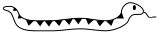
\includegraphics[width=.25\linewidth]{cute-snake-divider}
\end{center}
\vspace{.1em}
}
% Other divider lines I've tried out:
%\begin{center}\pgfornament[scale=.18]{85}\end{center}\vspace{.5em}
%\begin{center}\decorule\end{center}
%\vspace{1em}
%\fancybreak{\decofourleft \quad \decofourright}
%\vspace{1em}
%\begin{center}\emoji{thought-balloon}\end{center}
%\vspace{1em}
%\vspace{1em}
% SCHDEL:
%\usetikzlibrary{decorations.pathmorphing}
%\newcommand{\squigglyline}{
%\begin{center}
%\begin{tikzpicture}
%\pgfmathsetmacro\seglen{0.5*0.1}
%\draw [line width=0.4mm, decoration={snake, amplitude=1mm, segment length=\seglen\linewidth}, decorate] (0,0) -- (0.5\linewidth,0);
%\end{tikzpicture}
%\end{center}
%}

% Conditional probability: \textpr{foo}{bar} -> \Pr(\text{foo}\mid\text{bar})
%\newcommand{\probc}[2]{\ensuremath{\Pr(\text{#1}\mid\text{#2})}}

\hfuzz=2pt % Don't bother to report overfull hboxes if over-edge is < 2pt
\vfuzz=2pt % Same for overfull vboxes (maybe just works for hfuzz?)

%\newcommand{\BibTeX}{\rm B\kern-.05em{\sc i\kern-.025em b}\kern-.08em\TeX}

%%%%%%%%%%%%%%%%%%%%%%%%%%%%%%%%%%%%%%%%%%%%%%%%%%%%%%%%%%%%%%%%%%%%%%%%%%%%%%%%
%%%%%%%%%%%%%%%%%%%%%% TITLE, AUTHORS, ABSTRACT, KEYWORDS %%%%%%%%%%%%%%%%%%%%%%
%%%%%%%%%%%%%%%%%%%%%%%%%%%%%%%%%%%%%%%%%%%%%%%%%%%%%%%%%%%%%%%%%%%%%%%%%%%%%%%%

\newcommand{\longtitle}{The Snake Eyes Paradox}
\newcommand{\shorttitle}{Snake Eyes} % for page headers

\title{\HUGE\textbf{\longtitle}}
\author{Daniel M. Reeves\\manifold.markets/dreev
\and
Wamba Ivanhoe\\manifold.markets/ShitakiIntaki
}
\date{\protect\tstamp} % need protection from black magic, apparently

%\begin{abstract}
%The answer is 1/36.
%\end{abstract}

%\keywords{Probability, Math puzzles}

%%%%%%%%%%%%%%%%%%%%%%%%%%%%%%%%%%%%%%%%%%%%%%%%%%%%%%%%%%%%%%%%%%%%%%%%%%%%%%%%
%%%%%%%%%%%%%%%%% START DOCUMENT, SET UP HEADERS, DO MAKETITLE %%%%%%%%%%%%%%%%%
%%%%%%%%%%%%%%%%%%%%%%%%%%%%%%%%%%%%%%%%%%%%%%%%%%%%%%%%%%%%%%%%%%%%%%%%%%%%%%%%

\begin{document}
\pagestyle{headings}
\makeoddhead{headings}{\MakeUppercase{\shorttitle}}{}{\thepage}
\maketitle

%%%%%%%%%%%%%%%%%%%%%%%%%%%%%%%%%%%%%%%%%%%%%%%%%%%%%%%%%%%%%%%%%%%%%%%%%%%%%%%%
%%%%%%%%%%%%%%%%%%%%%%%%%%%%%%%% MAIN DOCUMENT %%%%%%%%%%%%%%%%%%%%%%%%%%%%%%%%%
%%%%%%%%%%%%%%%%%%%%%%%%%%%%%%%%%%%%%%%%%%%%%%%%%%%%%%%%%%%%%%%%%%%%%%%%%%%%%%%%

\chapter{Problem Statement}

You are offered a gamble.
A pair of six-sided dice are rolled and unless they come up snake eyes you get a bajillion dollars. 
If they do come up snake eyes, you're devoured by snakes.

So far it sounds like you have a 1/36 chance of dying, right?

Now the twist. 
First, I gather up an unlimited number of people willing to play the game, including you. 
I take 1 person from that pool and let them play. 
Then I take 2 people and have them play together, where they share a dice roll and either get the bajillion dollars each or both get devoured. 
Then I do the same with 4 people, and then 8, 16, and so on.

Eventually one of those groups will be devoured by snakes---hopefully not the group you're in---and then I stop.
Is the probability that you'll die, given that you're chosen to play, still 1/36?

\vspace{1em}

\textbf{Argument for NO:}
Due to the doubling, the final group of people that die is slightly bigger than all the surviving groups put together. 
So if you're chosen to play you have about a 50\% chance of dying!
\emoji{grimacing-face}
\emoji{snake}

\vspace{1em}

\textbf{Argument for YES:}
The dice rolls are independent and whenever you're chosen, what happened in earlier rounds is irrelevant.
Your chances of death are the chances of snake eyes on your round: 1/36.
\emoji{grinning-face-with-sweat}

\vspace{1em}

So which is it? 
What's your probability of dying, conditional on being chosen to play?
If you learn that your friend was chosen to play in this game and the game is now over, how worried are you?
If you wanted to play the one-shot version, do you still want to play the doubling groups version?

\vspace{1em}

\emph{Fine print: 
The game is not adversarial and the dice rolls are independent and truly random.
Groups are chosen uniformly and without replacement.
Void where prohibited.
}

\newpage

\chapter{Solution (With Limits)}

\iffalse
\begin{enumerate}
\item Choosing each group happens uniformly randomly.
\item This is technically undefined with an infinite pool of people but we can cap it and say that if no one has died after $N$ rounds then the game ends and no one dies. 
We just need to then find the limit as $N$ goes to infinity. 
%That way, instead of a 0\% chance of infinitely many people being chosen and none dying, we have a tiny chance of huge number of people being chosen and none dying.
% SCHDEL in which case the probability that no one dies goes to zero.
\item Importantly, in the finite version it's possible for no one to die. 
Just that the probability of that approaches zero as the size of the pool approaches infinity.
\item Again, we want the conditional probability that you die given that you are chosen to play.
In other words, of the people chosen, what fraction, in expectation, die?
In the unbounded case there's a 0\% chance of infinitely many people being chosen and none dying; in the bounded case it's a tiny chance of a huge number chosen and none dying.
\end{enumerate}
\fi


We want the probability that you die given that you are chosen to play, 
$\Pr(\text{death}\mid\text{chosen})$.
It seems like we can ignore the 0\% chance of rolling not-snake-eyes forever and say that eventually about half the people who are chosen die, but let's Bayes it out carefully:

\begin{equation*}
\begin{split}
\Pr(\text{death} \mid \text{chosen}) & =
\frac{\Pr(\text{chosen} \mid \text{death}) \Pr(\text{death})}{\Pr(\text{chosen})} \\
& = \frac{1\cdot\Pr(\text{death})}{\Pr(\text{chosen})}.
\end{split}
\end{equation*}

But if you're part of an infinite pool, you have a 0\% chance of being chosen and a 0\% chance of dying. 
The probability we want is 0/0. 
\emph{*robot-with-smoke-coming-out-of-its-ears-emoji*}

Since we can't directly calculate the probability in the infinite case, a natural thing to do is to take a limit.

\snakedivider

To get a feel for where we're going, suppose you're one person in a huge but finite pool.
Now suppose you are actually chosen. 
There are two ways that can happen: 
\begin{enumerate}
\item The pool runs out and everyone survives.
\item The pool doesn't run out and you have about a 50\% chance of dying. 
\end{enumerate}
But knowing that you are chosen is Bayesian evidence that we had many, many rounds of survival. 
If an early group died then most of the pool wasn't chosen, so probably you weren't chosen.

Thinking like a Bayesian means shifting your probability in light of evidence by seeing how surprised you'd be in various universes by that evidence.
If an early group died then most people aren't chosen and in that universe you're surprised to be chosen. 
If \emph{no} group died then everyone was chosen and in that universe you're fully unsurprised that you were chosen. 
That's the sense in which being chosen is Bayesian evidence that more people survived. 
In particular it's at least weak evidence that everyone survived.

So even with an absurdly huge pool of people, where there's \emph{essentially} a 0\% chance of everyone surviving, if you know you were chosen (which itself has near zero probability, but, you know, \emph{if}) then that means you're more likely to be in that essentially-0\%-probability universe where everyone survives.

\snakedivider

Enough hand-waving and appeals to intuition.
Let's Bayes it out to see what 
$\Pr(\text{death} \mid \text{chosen})$
is exactly, in a finite version where we stop after $N$ rounds.
Once we have that, we can take the limit as $N$ goes to infinity.

First, let $M$ be the size of the pool:

$$M = \sum_{i=1}^{N} 2^{i-1} = 2^N-1.$$

And let $p$ be the probability of snake eyes, 1/36.
We can now compute the probability of being chosen by summing up 
(1) the probability you're chosen for the first round, $1/M$, plus 
(2) the probability that the first group survives, $1-p$, and that you're chosen for the 2nd round, $2/M$, plus 
(3) the probability that the first two groups survive and you're chosen for the 3rd round, etc.
Writing that out as an equation gives this:

\begin{align*}
\Pr(\text{chosen}) & = 
\begin{aligned}[t]
\tfrac{1}{M} & + (1-p)      \tfrac{2}{M} \\
             & + (1-p)^2    \tfrac{4}{M} \\
             & + (1-p)^3    \tfrac{8}{M} \\
             & + \ldots                  \\
             & + (1-p)^{N-1}\frac{2^{N-1}}{M}
\end{aligned} \\
& = \sum_{i=1}^{N} \tfrac{1}{M} 2^{i-1}(1-p)^{i-1}.
\end{align*}

For $\Pr(\text{death})$ the calculation is very similar but every term is multiplied by $p$.
To die, you have to be chosen and then roll snake eyes.
This can happen on any round, all of which are mutually exclusive.
We can then factor that $p$ out and we have

$$
\Pr(\text{death}) = p\cdot\Pr(\text{chosen}).
$$

Working out that expression for $\Pr(\text{chosen})$ wasn't even necessary!
We compute $\Pr(\text{death} \mid \text{chosen})$ like so:
\begin{equation*}
\begin{split}
\Pr(\text{death} \mid \text{chosen}) & = 
\frac{\Pr(\text{death})}{\Pr(\text{chosen})} \\
& = \frac{p\cdot\Pr(\text{chosen})}{\Pr(\text{chosen})} = 
p.
\end{split}
\end{equation*}

It doesn't depend on $N$ at all!
The limit as $N$ goes to infinity is just... 
$p$ or 1/36, the probability of rolling snake eyes.
\qedsymbol{}

%\chapter*{Discussion and Dead-Horse Beating}
\chapter{Can We Roll Not-Snake-Eyes Forever?}

What about the argument that, with unlimited people, there will necessarily be a finite round $n$ at which snake eyes is rolled?
And for every possible such $n$, at least half of the chosen players die.
After all, the probability of rolling not-snake-eyes forever is zero. 
(More precisely, in the limit as $n$ goes to infinity, the probability of rolling not-snake-eyes $n$ times in a row goes to zero.)

That's all true but let's work out the probability of rolling not-snake-eyes forever \emph{conditional on you being chosen}.
Starting with $\Pr(\text{snake eyes})$ as the probability that a game rolls snake eyes---unambiguously 1---we have, by the definition of conditional probability:
\begin{equation*}
\Pr(\text{snake eyes} \mid \text{chosen})
= \frac{\Pr(\text{chosen} \land \text{snake eyes})}{\Pr(\text{chosen})}.
\end{equation*}

In the infinite setting that's
$\tfrac{0}{0}$
because you have a 0\% chance of being chosen from an infinite pool.
So let's work it out in the limit with a cap of $N$ rounds and finite pool $M$ as before:
$$\dfrac
{\sum\limits_{i=1}^{N}(1-p)^{i-1}p \cdot\dfrac{2^i-1}{M}}
{\sum\limits_{i=1}^{N}\tfrac{1}{M} 2^{i-1}(1-p)^{i-1}}.
$$
In the numerator we're summing over every possible round $i$ at which we could roll snake eyes, saying that we need to roll not-snake-eyes $i-1$ times followed by one snake eyes \emph{and} that we are chosen in any round from 1 through $i$.
The denominator, $\Pr(\text{chosen})$, is the same as in the previous section.

Now algebra ensues.
We multiply the numerator and denominator by $M$ to get rid of the $1/M$ factor, 
%$$\dfrac
%{\sum\limits_{i=1}^{N} (1-p)^{i-1}p \cdot(2^i-1)}
%{\sum\limits_{i=1}^{N} 2^{i-1}(1-p)^{i-1}}.
%$$
then distribute the $(1-p)^{i-1}p$ over the $2^i-1$ and split it into two summations:
$$\dfrac{
\left(\sum\limits_{i=1}^{N}2^i(1-p)^{i-1}p\right) -
\left(\sum\limits_{i=1}^{N}(1-p)^{i-1}p \right)
}{\sum\limits_{i=1}^{N} 2^{i-1}(1-p)^{i-1}}.
$$
These are finite sums so that's kosher.
The right side of the numerator is the probability of rolling snake eyes by round $N$, which is $\Pr(\text{snake eyes})$ in the limit as $N$ goes to infinity, so we replace that sum by one:
$$\dfrac{
\left(\sum\limits_{i=1}^{N}2^i(1-p)^{i-1}p\right) - 1
}{\sum\limits_{i=1}^{N}2^{i-1}(1-p)^{i-1}}.
$$
Almost there!
Pull a $2p$ out of the sum in the numerator to get this:
$$\dfrac{
2p\left(\sum\limits_{i=1}^{N}2^{i-1}(1-p)^{i-1}\right) - 1
}{\sum\limits_{i=1}^{N}2^{i-1}(1-p)^{i-1}}.
$$
Notice that the sums in the numerator and denominator are now identical.
We distribute the denominator,
$$2p - \dfrac{1} 
{\sum\limits_{i=1}^{N}2^{i-1}(1-p)^{i-1}},
$$
and combine the terms in the sum,
$$2p - \dfrac{1} 
{\sum\limits_{i=1}^{N}\left(2(1-p)\right)^{i-1}},
$$
to see that the denominator is a finite geometric series with common ratio $2(1-p)$.
As long as the common ratio is greater than or equal to 1, 
%(i.e., $p\leq 1/2$ which for us is the case, namely $p=1/36$), 
the denominator diverges and the above approaches $2p$ in the limit as $N$ goes to infinity.
How do we know $2(1-p) \geq 1$?
Because we can rearrange it as $p\leq 1/2$ and that's true for us, namely $p=1/36$.\footnote{
What would happen if we had $p>1/2$?
In that case, by the preceding derivation, $\Pr(\text{snake eyes} \mid \text{chosen}) = 1$ so no chance of everyone surviving.
That makes sense because the whole paradox is ruined if $p>1/2$.
The probability of dying in the one-shot version is already greater than the fraction of people who die when the game ends in snake eyes.}

In conclusion, the probability of eventually rolling snake eyes, conditional on you being chosen to play, approaches $2p=1/18$ in the limit.
Which is to say that the conditional probability of rolling not-snake-eyes literally forever is $17/18$.
\emoji{exploding-head}

(Or to say it less sensationally: For any finite $N$, the conditional probability of taking more than $N$ rolls to hit snake eyes is greater than $17/18$.)

This vindicates our initial intuitive argument that being chosen is Bayesian evidence---strong Bayesian evidence, it turns out!---of never rolling snake eyes.
And it invalidates the intuition that we can safely condition on snake eyes being rolled just because it definitely will be rolled (unconditionally).
Another version of that intuition is that any event with probability 1, such as rolling snake eyes eventually, must be independent of any other event.
%When we condition upon this zero measure event, we can no longer assume that rolling snake eyes is independent from being chosen!
But if being chosen and rolling snake eyes were independent then, by definition of independence,
$\Pr(\text{chosen} \land \text{snake eyes}) = \Pr(\text{chosen})\cdot\Pr(\text{snake eyes})$.
And if that were true, we'd conclude from the above derivation of $\Pr(\text{snake eyes}\mid\text{chosen})$ that
\begin{align*}
   & \Pr(\text{snake eyes})\\
 = & \frac{\Pr(\text{chosen})\Pr(\text{snake eyes})}{\Pr(\text{chosen})}\\
 = & \frac{\Pr(\text{chosen} \land \text{snake eyes})}{\Pr(\text{chosen})}\\
 = & \Pr(\text{snake eyes}\mid\text{chosen})\\
 = & 1/18.
\end{align*}
Which contradicts $\Pr(\text{snake eyes}) = 1$.
%So within the context of conditioning upon being chosen, these two events cannot be independent.
The temptation to treat $\Pr(X)$ as $\Pr(X \mid \text{snake eyes})$ since $\Pr(\text{snake eyes}) = 1$ leads us astray!

%\appendix

%\part*{Appendices}

\chapter{To Infinity And Beyond (With A Nonuniform Prior)}

What if we reject the whole idea of defining a finite version of Snake Eyes to take a limit of?
Can we math out an answer for the infinite game directly?
Yes!
The only monkey wrench is that we can't have a uniform prior over an infinite set.\footnote{
Not in standard analysis anyway.
If infinitely many things are all equally likely then they all have zero probability.
Or to be slightly more formal, there's an elegant proof by contradiction:
First, the sum of the probabilities of each element of the set must be $1$.
That's part of what it means to have a prior over a set of possibilities.
Now suppose every element in your infinite set has equal probability $\epsilon$.
That's what we mean by a uniform prior.
Further suppose that $\epsilon=0$.
Then the sum of the probabilities is $0$.
So that's no good; we must have $\epsilon>0$.
But the sum of an infinite number of positive $\epsilon$'s is infinity.
So that's no good either.
$\rightarrow\leftarrow$
}
So let's just say we don't \emph{quite} have a uniform prior.
Maybe you think you're equally likely to be any of the first trillion people chosen to play and that it gradually becomes less likely after that.
We can make that "trillion" as high as we like.

As long as the probability of being chosen isn't exactly zero, there's no division-by-zero problem like before.

Is that fair though, to reject the stipulation in the problem statement that you're chosen uniformly?
Well, it's arguably less of a leap than we made before in defining a finite version of the game where it's possible for no one to die.
We're just saying you're not quite chosen uniformly because you \emph{can't} be and have any probability of being chosen at all.
But we can get arbitrarily close to uniform!
We can even consider the limit as the distribution approaches uniform.
Great, let's get to it!

Let $\text{CH}_c$ be the event that you're chosen to play in round $c$ and let $\text{SE}_s$ be the event that snake eyes is rolled in round $s$.
Define 
$p_{cs} = \Pr(\text{CH}_c\land \text{SE}_s)$ 
as the probability of a game where you're chosen in round $c$ and snake eyes is rolled in round $s$.
In this formulation, $\text{CH}_c$ and $\text{SE}_s$ are independent for all $c$ and $s$.
So $c>s$ is possible, just that it means a game where you're not chosen because snake eyes was rolled before we got to you.
Summing $p_{cs}$ over every possible $c$ and $s$---every possible game---necessarily gives us 1:
$$
\sum_{s=1}^\infty \sum_{c=1}^\infty p_{cs} = 1.
$$

The independence of $\text{CH}_c$ and $\text{SE}_s$ gives us the following:
\begin{align}\label{pcs}
\begin{split}
p_{cs} & = \Pr(\text{CH}_c\land\text{SE}_s) \\
       & = \Pr(\text{CH}_c)\cdot\Pr(\text{SE}_s) \\
       & = \Pr(\text{CH}_c)\cdot(1-p)^{s-1}\cdot p.
\end{split}
\end{align}
That final line is because the only way to get snake eyes on round $s$ is by rolling not-snake-eyes $s-1$ times in a row followed by one snake eyes.

We can write the unconditional probability of death like this:
\begin{equation}\label{d}
\Pr(\text{death}) = \sum_{i=1}^\infty p_{ii}.
\end{equation}
That's just summing up all the infinite ways you can be chosen on the same round that snake eyes is rolled.

For the unconditional probability of being chosen to play, we can get it two ways:
\begin{equation}\label{c}
\Pr(\text{chosen}) = 
\sum_{s=1}^\infty\sum_{c=1}^s p_{cs} =
\sum_{c=1}^\infty\sum_{s=c}^\infty p_{cs}.
\end{equation}
In the first double sum, the outer sum iterates over every round $s$ on which we might roll snake eyes and the inner sum covers all the cases where you're chosen on or before $s$.
In the second double sum, the outer sum iterates over every round $c$ in which you can be chosen and the inner sum covers all the cases where snake eyes is rolled on or after $c$.

Eventually we want to find the probability of death given that you're chosen.
As we saw in the original derivation, Bayes' Law tells us that this is 
$\Pr(\text{death}) / \Pr(\text{chosen})$.
But first let's compute $\Pr(\text{death}\mid\text{CH}_c)$, your probability of death given that you're chosen on a particular round $c$.
We expect that to be $p=1/36$ because it amounts to the one-shot scenario:
a specific round $c$ when you're chosen means there's exactly one way to die, namely, rolling snake eyes on that specific round.
To be totally sure, and to sanity-check our $p_{cs}$ definition, let's now compute it rigorously.
We start with the definition of conditional probability:
$$
\Pr(\text{death}\mid\text{CH}_c) = 
\frac{\Pr(\text{death}\land\text{CH}_c)}{\Pr(\text{CH}_c)}.
$$
The numerator can also be written $\Pr(\text{SE}_c\land\text{CH}_c)$ or
$p_{cc}$, the probability that you're both chosen in round $c$ and that snake eyes is rolled on round $c$.
And we can write the denominator in terms of $p_{cs}$ by summing over all the ways you can be chosen in round $c$:
\begin{equation}\label{cc}
\frac{p_{cc}}{\sum\limits_{s=c}^\infty p_{cs}}.
\end{equation}

Now we use~\eqref{pcs} to expand that to
$$
\frac{\Pr(\text{CH}_c)\cdot(1-p)^{c-1}\cdot p}{\sum\limits_{s=c}^\infty \Pr(\text{CH}_c)(1-p)^{s-1} p}
$$
and cancel common factors (notice we're summing over $s$, not $c$) to get this:
$$
\frac{(1-p)^{c-1}}{\sum\limits_{s=c}^\infty (1-p)^{s-1}}.
$$
Because the denominator is a geometric series starting at $(1-p)^{c-1}$ and with common ratio $1-p$ we can replace it with its closed form and simplify the above to this:
$$
\frac{(1-p)^{c-1}}{\frac{(1-p)^{c-1}}{p}}.
$$
And that simplifies to $p$.
Phew!

Knowing that~\eqref{cc} equals $p$ implies that
\begin{equation}\label{s}
\sum\limits_{s=c}^\infty p_{cs} = \frac{p_{cc}}{p}.
\end{equation}

Finally we have everything we need to work out your chances of dying if you're chosen to play.
Recall that
\begin{align*}
\Pr(\text{death} \mid \text{chosen}) 
& = \frac{\Pr(\text{chosen} \mid \text{death}) \Pr(\text{death})}{\Pr(\text{chosen})} \\
& = \frac{\Pr(\text{death})}{\Pr(\text{chosen})}. \\
\end{align*}
By~\eqref{d} and~\eqref{c}, that becomes
$$
\frac{\sum\limits_{i=1}^\infty p_{ii}}{\sum\limits_{c=1}^\infty\sum\limits_{s=c}^\infty p_{cs}}.
$$
Coup de gr\^ace coming up.
The inner sum in the denominator is the left-hand side of~\eqref{s} so we can substitute that in like so:
$$
\frac{\sum\limits_{i=1}^\infty p_{ii}}{\sum\limits_{c=1}^\infty\frac{p_{cc}}{p}}.
$$
And we're home free.
Factor out the $1/p$ and the sums are the same sum:
$$
\frac{\sum\limits_{i=1}^\infty p_{ii}}{\frac{1}{p}\sum\limits_{c=1}^\infty p_{cc}}.
$$
They cancel and the $1/p$ flips to the top as $p$ and we're done! \qed

Amazingly, we didn't need to define a finite version of the game.
We just need a valid prior on when you're chosen.
And even more amazingly, the answer is completely independent of what that prior is.
For example, say it's uniform for the first $N$ possible values of where you are in the queue of people in the pool.
Now compute $\Pr(\text{death}\mid\text{chosen})$ in terms of $N$.
The answer, as we just saw, is $p$.
No $N$ in sight.
So in the limit as our prior approaches uniform?
Still $p$.

Or maybe you don't like that the above prior has a finite cutoff.
No problem.
Here's a prior that's both arbitrarily close to uniform and puts positive probability on all infinitely many future rounds in which you could be picked:
\begin{itemize}
\item Your probability of being chosen first is 1 in a million
\item Your probability of being $n$th in the queue is 99.9999\% as much as your probability of being $n-1$st.
\end{itemize}
In the limit as that "million" goes to infinity (and the 99.9999\% correspondingly goes to 1) we again have a uniform prior.
Paradox: resolved and double-resolved.

\end{document}

\chapter*{Appendix: Response to NO, Wamba's Version}

%$p_{cs}$

Let $\Pr(i,j)$ be the mutually exclusive absolute odds of an individual being selected in Round $i$ of a game that rolls snake eyes in Round $j$. 
Since the game ends the round that we roll snake eyes we have $i\leq j \text{ }\forall \text{ } i\text{,}j \in \mathbf{N}$. 
If $i > j$ then we were not selected because the game ended before we could play. 
When $i=j$ then we are devoured by snakes.
The absolute odds of dying is found by adding up all the possible games where we are selected in the final round:
\begin{equation}
  \sum_{j=1}^{\infty} \Pr(j,j) \label{die}
\end{equation} 
The absolute odds of being chosen are the games where  $i\leq j \text{ }\forall \text{ } i\text{,}j \in \mathbf{N}$:
\begin{equation}
  \sum_{j=1}^{\infty} \sum_{i=1}^{j} \Pr(i,j) = \sum_{i=1}^{\infty} \sum_{j=i}^{\infty} \Pr(i,j) \label{chosen} 
\end{equation}

The odds of dying, conditioned upon being selected is simply the ratio of \ref{die} over \ref{chosen}
\begin{equation}
  \frac{\sum_{j=1}^{\infty} \Pr(j,j)}{\sum_{j=1}^{\infty} \sum_{i=1}^{j} \Pr(i,j)}\label{theAnswer}
\end{equation}

NO asserts that the following is the odds of dying, conditioned upon being selected:
\begin{align*}
& \sum_{j=1}^{\infty} \frac{\Pr(j,j)p(1-p)^{j-1}}{\sum_{i=1}^{j} \Pr(i,j)} \\
= & \frac{1}{1}p + \frac{2}{3}p(1-p) + \frac{4}{7}p(1-p)^2 + ... \\
\approx & 0.5218873
\end{align*}

It is generally accepted that 
$$\frac{\sum_{i=1}^{n} a_i}{\sum_{i=1}^{n} b_i}\nLeftrightarrow \sum_{i=1}^{n} \frac{a_i}{b_i}$$

However we do know that if 
$$\frac{a_i}{b_i}=\frac{a_j}{b_j} \text{   } \forall \text{ } i\text{,}j \in \{1...n\}$$
then
$$\frac{\sum_{i=1}^{n} a_i}{\sum_{i=1}^{n} b_i} = \frac{a_j}{b_j}\text{   } \forall \text{ } i\text{,}j \in \{1...n\}$$

The local odds of dying knowing only that you are selected in Round $i$ and that the game may or may not continue is $p$.  This makes sense since with the locally known information it is just like you are playing a one shot game, observing just one roll of the dice.  Which means
$$\frac{\Pr(i,i)}{\sum_{j=i}^{\infty}\Pr(i,j)} = p \text{  }\forall \text{  } i \in \mathbf{N}$$
which, once accepted, is enough to show that \ref{theAnswer} is also $p$
$$ \frac{\sum_{j=1}^{\infty} \Pr(j,j)}{\sum_{j=1}^{\infty} \sum_{i=1}^{j} \Pr(i,j)} = \frac{\sum_{i=1}^{\infty}\Pr(i,i)}{\sum_{i=1}^{\infty}\sum_{j=i}^{\infty}\Pr(i,j)} = p $$

So lets algebra out the probability of losing, if you are chosen in Round i.
We said that $\Pr(i,j)$ is the mutually exclusive absolute odds of an individual being selected in Round $i$ of a game that rolls snake eyes in Round $j$.  We might need to say what that looks like algebraically. 
\begin{equation}
  \Pr(i,j) = \frac{2^i}{M}p(1-p)^{j-1}
\end{equation}
M is a placeholder for the population size and $2^i$ is the number of players in Round $i$.  $p(1-p)^{j-1}$ is the probability that the game rolls $j-1$ non-snake-eyes before rolling snake eyes on Round $j$

It is only possible to be chosen to play in Round $i$ if $i\leq j$.  You die when $j=i$ otherwise you live for all $j>i$. 
\begin{align*}
 &= \frac{\Pr(i,i)}{\sum_{j=i}^\infty \Pr(i,j)}\\
 &=\frac{\frac{2^{i}p(1-p)^{i-1}}{M}}{\sum_{n=i}^{\infty} \frac{2^{i}p(1-p)^{n-1}}{M}}\\
 &=\frac{p(1-p)^{i-1}}{\sum_{n=i}^{\infty}p(1-p)^{n-1}}\\
 &=\frac{p(1-p)^{i-1}}{p\frac{(1-p)^{i-1}}{1-(1-p)}}\\
 &=\frac{p(1-p)^{i-1}}{(1-p)^{i-1}}\\
 &=p
\end{align*}
Ergo the probability of dying, conditional on being chosen is $p$.

\wamba{
This should makes sense to us within the narrative that, if you are selected to play in any specific round then the odds of you losing that round is determined by a fair dice roll made for that round and your odds of losing are $p=\frac{1}{36}$. No matter which round you are selected to play in, if you play you will only observe one roll of the dice and, since the dice rolls are independent, the process and your observation are memory-less.
}

\end{document} % END HERE FOR LORXUS SUBMISSION

\vspace{2em}
\noindent
\emph{Source: This is a variant of the Shooting-Room Paradox.
Googling that yields a sea of confusion and wrongness and paywalled philosophy papers so we wrote this.}

%%%%%%%%%%%%%%%%%%%%%%%%%%%%%%%%%%%%%%%%%%%%%%%%%%%%%%%%%%%%%%%%%%%%%%%%%%%%%%%%

\chapter*{Acknowledgments}

Thanks to 
Greta Goodwin, 
Bethany Soule, 
Christopher Moravec,
and Stan Wagon, as well as
CesiumLifeJacket and Nix and others in the PEAR Discord for helpful discussion.

Thanks also to Manifold Markets where we
\href{https://manifold.markets/dreev/is-the-probability-of-dying-in-the}{posed this question}.
The market converged to the correct answer amidst heated discussion in the comments:

\vspace{2em}
\noindent
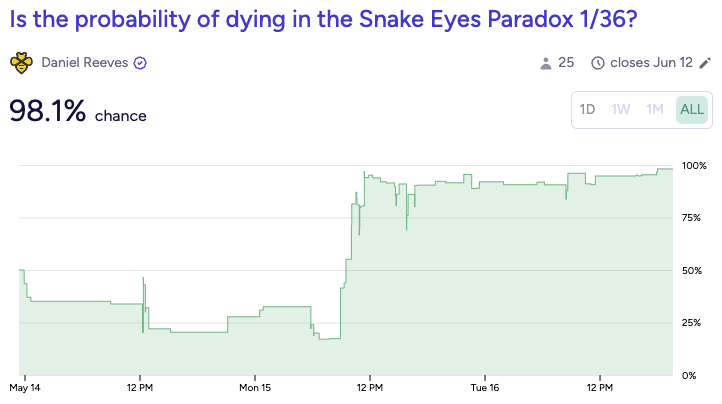
\includegraphics[width=\linewidth]{manifold-snakeeyes}


% random unrelated thing i wanted rendered:
%$$
%\mathop{\mathrm{arg\,max}}_{a \in \text{Actions}} \text{EU}(a)
%$$

\newpage
\newpage

\chapter{Wamba's Writeup}

\emph{(Dreev and Wamba are currently working on merging their writeups. For now, Dreev's is before this point and Wamba's is after.)}

The title of the Manifold Market is 
\textbf{"Is the probability of dying in the Snake Eyes Paradox 1/36?"} 
which is not posed as a question of a conditional probability.
Indeed the intent is to ask about a probability conditioned upon being chosen to play, and there has been some confusion about whether the question in the description is conditional or a further restriction:

Is the probability that you'll die [in the Snake Eyes Paradox], given that you're chosen to play, still 1/36?

So I hope it is clear to the reader, that we are asking questions about conditional probabilities and so I will try to pose my conditional questions in a format of "Question, if Conditional" i.e.

Is the probability that you'll die in the Snake Eyes Paradox, if you're chosen to play, 1/36?

\section{Groundwork}
Bayes Theorem in the context of the question asked in the Snake Eye's market.
\[\Pr(\text{death}|\text{chosen}) = \frac{\Pr(\text{chosen}|\text{death})\Pr(\text{death})}{\Pr(\text{chosen})}\]
Here we observe that $\Pr(\text{chosen}|\text{death})$ must equal 1, because you can't die in the game if you weren't chosen to play, so the conditional probability we seek simplifies to 
\begin{equation}\label{eq:D|C_primative}\Pr(\text{death}|\text{chosen})=\frac{\Pr(\text{death})}{\Pr(\text{chosen})}\end{equation}
For my proof we will construct upon first a finite population of willing players $M$ which we will say supports at most $m$ rounds of Snake Eyes play.
First we will look at the probability mass of the game ending in round $i$, where the initial round is $i=0$.
For those games that end because snake eyes was rolled, the snake eyes was rolled with a probability $p$ and $i$ non-snake eyes were rolled with probability $(1-p)^{i}$ so we will denote the probability of ending with snake eyes in round $E=i$ as
\[\Pr(E=i) = p(1-p)^{i} \]
For this to be a full probability mass function on our population size $M$ we should find that the sum across rounds 0 to $m-1$ equals 1
$$\sum_{i=0}^m-1 p(1-p)^{i} = p\frac{1 - (1-p)^m}{1 - (1-p)} = 1-(1-p)^m$$
We can see that this sum is strictly less than 1 by a term of $(1-p)^m$ which coincides exactly with the probability mass of rolling non-snake eye $m$ times in a row.  The case where after $m$ rounds no one has lost the game.
So our full probability mass distribution for a population $M$ is comprised of $m$ cases where the game ends in snake eyes and one case where there are no snake eyes.  This $(1-p)^m$ term is keeping track of what is happening after $m$ rounds have been played, in the finite case we stop playing and no one dies, in the limit to $\infty$ this term is is keeping track of what happens to the game that no one dies in, a game that goes on for infinitely many rounds. 
\[1 = (1-p)^ m + \sum_{i=0}^m p(1-p)^{i} \]

Next lets look at the probability mass distribution for probability that a player plays in round $j$, starting at $j=0$ for the first round.  The first round has 1 player and each subsequent round has twice as many players and the round preceding it so the probability that a player is chosen in round $C=j$ we will denote as  
\[\Pr_M(C=j) = \frac{2^j}{M}\]
This probability mass distribution is dependent upon the size of our population so we denote the $\Pr$ with a subscript $M$. If $\Pr_M(C)$ is going to represent the full probability space it must sum to 1 across all possible $j$ for population size $M$.
\[\sum_{j=0}^{m-1}  \frac{2^j}{M} = \frac{2^m - 1}{M}\]
If $M\neq 2^m - 1$ then we will have a bucket where the probability mass of not being chosen at all to play must equal $1-\frac{2^m-1}{M}$.
With our final bucket of $1-\frac{2^m-1}{M}$ we now have two independent probability mass distribution functions which each sum to 1 when we iterate their index over the set $\{0,...,m-1\}$ which we will use to populate a Bayes Probability Table to see the terms of the joint probability mass distribution $Pr_M(E=i,C=j)$. 
See Figure \ref{fig:BayTable}.

\begin{figure*}
    \begin{center}
        \caption{Consider the Bayes Probability Table for an arbitrary finite population  $M$.}
        \label{fig:BayTable}
        \begin{tabular}{ r | c c c c c c | }
            $Pr_M(E,C)$ & $\frac{1}{M}$ & $\frac{2}{M}$ & $\frac{4}{M}$ & $...$ & $\frac{2^{m -1}}{M}$ & $1-\frac{2^m-1}{M}$\\
            \hline
            $p$ & \cellcolor{red!25}$\frac{p}{M}$ & \cellcolor{yellow!25}$\frac{2p}{M}$ & \cellcolor{yellow!25}$\frac{4p}{M}$ & \cellcolor{yellow!25}$...$ & \cellcolor{yellow!25}$\frac{2^{m -1}p}{M}$ & \cellcolor{yellow!25}$p(1-\frac{2^m-1}{M})$\\ 
            $p(1-p)$ & \cellcolor{green!25}$\frac{p(1-p)}{M}$ & \cellcolor{red!25}$\frac{2p(1-p)}{M}$ & \cellcolor{yellow!25}$\frac{4p(1-p)}{M}$ & \cellcolor{yellow!25}$...$ & \cellcolor{yellow!25}$\frac{2^{m -1}p(1-p)}{M}$ & \cellcolor{yellow!25}$p(1-p)(1-\frac{2^m-1}{M})$\\ 
            $p(1-p)^2$ & \cellcolor{green!25}$\frac{p(1-p)^2}{M}$ &\cellcolor{green!25} $\frac{2p(1-p)^2}{M}$ & \cellcolor{red!25}$\frac{4p(1-p)^2}{M}$ & \cellcolor{yellow!25}$...$ & \cellcolor{yellow!25}$\frac{2^{m -1}p(1-p)^2}{M}$& \cellcolor{yellow!25}$p(1-p)^2(1-\frac{2^m-1}{M})$ \\ 
            $\vdots$ & \cellcolor{green!25}$\cellcolor{green!25}\vdots$ & \cellcolor{green!25}$\vdots$ & \cellcolor{green!25}$\vdots$ & \cellcolor{red!25}$\ddots$ & \cellcolor{yellow!25}$\vdots$& \cellcolor{yellow!25}$\vdots$ \\
            $p(1-p)^{m-1}$ & \cellcolor{green!25}$\frac{p(1-p)^{m-1}}{M}$ & \cellcolor{green!25}$\frac{2p(1-p)^{m-1}}{M}$ & \cellcolor{green!25}$\frac{4p(1-p)^{m-1}}{M}$ & \cellcolor{green!25}$...$ & \cellcolor{red!25}$\frac{2^{m -1}p(1-p)^{m-1}}{M}$& \cellcolor{yellow!25}$p(1-p)^{m-1}(1-\frac{2^m-1}{M})$ \\ 
            $(1-p)^m$ & \cellcolor{green!25}$\frac{(1-p)^m}{M}$ & \cellcolor{green!25}$\frac{2(1-p)^m}{M}$ & \cellcolor{green!25}$\frac{4(1-p)^m}{M}$ &\cellcolor{green!25} $...$ & \cellcolor{green!25}$\frac{2^{m -1}(1-p)^m}{M}$& \cellcolor{yellow!25}$(1-p)^m(1-\frac{2^m-1}{M})$ \\ 
            \hline
        \end{tabular}
    \end{center}
\end{figure*}

%%%%%%%%%%%
%% Might just drop this figure 2, doesn't add much and really messes with the rest of the lay out.
%  What are your thoughts Dreev?
%%%%%%%%%%%
%not presently redering because of the [H] option
\begin{figure*}[H]
    \begin{center}
    \caption{The cells we are interested in from Figure \ref{fig:BayTable} can be abstracted to cases with snake eyes in round $i$ or no snake eyes.}
    \label{fig:TableLite}
        \begin{tabular}{ r | c  c |}
        $Pr_M(E=i,C=j)$ & $\frac{2^j}{M}$ & $\sum_{j=0}^{m-1}\frac{2^j}{M}$ \\
        \hline
        $p(1-p)^{i}$ & $\frac{2^{j}p(1-p)^{i}}{M}$ & \\ 
        $(1-p)^m$ & & \cellcolor{green!25}$\frac{(2^{m }-1)(1-p)^m}{M}$ \\ 
        \hline
        \end{tabular}
    \end{center}
\end{figure*}
%% The color boxes are cute, but they also make this paragraph typset differntly than the rest of the paper  Probably can get rid of the color.
Here we can note if 
\colorbox{red!25}{$i=j$ then the player lost}.
If \colorbox{green!25}{$j<i$ then the player won} 
in an earlier round before the game ended in snake eyes. 
In either of these cases ($j\leq i$) and the player was chosen. 
We also note that game where no snake eyes are ever rolled at is the 
\colorbox{green!25}{bottom row} and 
\colorbox{green!25}{everyone is chosen and wins} 
in such a game.
Finally if 
\colorbox{yellow!25}{$j>i$ then the player was not chosen} 
because the game ended before the player could be chosen. 




\section{What is the probability of losing?}
All we need to do is sum the probabilities $Pr_M(E=i,C=j)$ where $i=j$,  $$\Pr_M(\text{death}) =
\sum_{i=0}^{m-1} \frac{2^{j}p(1-p)^{i}}{M}$$
We factor out $p$ and $M$ which are constant and substitute $i=j$ to arrive at 
\begin{equation}
\label{eq:D}
\Pr_M(\text{death})= \frac{p}{M}\sum_{i=0}^{m-1} 2^{i }(1-p)^{i}
\end{equation}
%%%%%%%%  This can probably go, it is excessive, but demonstrates that 0/0 can = p if we have taken the time to property model.  Trivial for a mathematician perhapse.  All of this algebra is highschool level to help the regular market trader on manifold follow along.
Note that the limit of $\Pr_M(\text{death})$ is zero as $M$ and $m$ go to infinity.
\begin{align*}
    \lim_{m\to\infty}  & \frac{p}{M}\sum_{i=0}^{m-1} 2^{i }(1-p)^{i}\\
    = \lim_{m\to\infty}  & \frac{p}{M}\bigg(\frac{1-2^m(1-p)^m}{1-2(1-p)}\bigg)\\
    =\lim_{m\to\infty}  & \frac{p}{2p-1}\bigg(\frac{1-2^m(1-p)^m}{M}\bigg)\\
    & M \geq 2^m-1\\
    \leq \lim_{m\to\infty}  & \frac{p}{2p-1}\bigg(\frac{1-2^m(1-p)^m}{2^m-1}\bigg)\\
    =\lim_{m\to\infty}  & \frac{p}{2p}\bigg(\frac{-2^m(1-p)^m}{2^m}\bigg)\\
    =\lim_{m\to\infty}  & \frac{-(1-p)^m}{2} = \frac{0}{2} = 0\\
\end{align*}





\section{What is the probability of being chosen?}
Here we require the sum of the probabilities $Pr_M(E=i,C=j)$ where $i\geq j$ as well as the probability that the game never rolls snake eyes.
Note that the contribution from the bottom row is $\sum_{j=0}^{m-1} \frac{2^{j}(1-p)^m}{M}$ accounts for being selected in the game that ends with out rolling snake eyes so we just need to sum up the rest of the probabilities contributed by the games that do end in snake eyes.
\begin{align*}
  \Pr_M(\text{chosen})=& \\
=&\sum_{j=0}^{m-1} \frac{2^{j}(1-p)^m}{M} + \sum_{i=0}^{m-1}\sum_{j=0}^{i} \frac{2^jp(1-p)^i}{M}
\end{align*}

Again $p$ and $M$ are constants and can be factored out from the double summation and the $(1-p)^i$ factor is a constant with respect to the summation over index $j$ so we can factor that out from the $j$ summation.
\begin{align*}
 = & \ \ \frac{(1-p)^m}{M}\sum_{j=0}^{m-1}2^{j} + \frac{p}{M}\sum_{i=0}^{m-1} (1-p)^i\sum_{j=0}^{i} 2^j\\
 = & \ \ \frac{1}{M} \ \big[ \ (2^m-1)(1-p)^m   \\
    & \ \ \   + p\sum_{i=0}^{m-1} (1-p)^{i}(2^{i+1}-1) \ \big]\\
= & \ \ \frac{1}{M} \ \big[ \  (2^m-1)(1-p)^m    \\
    & \ \ \ + p\sum_{i=0}^{m-1}2^{i+1}(1-p)^{i}    \\
    & \ \ \ -p\sum_{i=0}^{m-1} (1-p)^{i} \ \big]
\end{align*}  %%%%%%%%%%%%%%%% Manual Column Break Assistance %%%%%%%%%%%
\begin{align*}  %%%%%%%%%%%%%%%%%%%%%%%%%%%%%%%%%%%%%%%%%%%%%%%%%%%%%%%%%
 = & \ \ \frac{1}{M} \ \big[ \ (2^m-1)(1-p)^m    \\
    & \ \ \  + 2p\sum_{i=0}^{m-1}2^{i}(1-p)^{i}    \\
    & \ \ \ -p\sum_{i=0}^{m-1} (1-p)^{i} \ \big]    \\
= &  \ \ \frac{1}{M} \ \big[ \   (2^m -1)(1-p)^m  &\\
    & \ \ \ + \sum_{i=0}^{m-1}2^{i}(1-p)^{i} &\\
    & \ \ \ +(2p-1)\sum_{i=0}^{m-1}2^{i}(1-p)^{i} & \\ 
    & \ \ \ -p\sum_{i=0}^{m-1} (1-p)^{i}  \ \big]\\
= & \ \ \frac{1}{M} \ \big[ \   2^m(1-p)^m -(1-p)^m  &\\
    & \ \ \ + \sum_{i=0}^{m-1}2^{i}(1-p)^{i} &\\
    & \ \ \  +(2p-1)\frac{1-2^{m}(1-p)^{m}}{1-2(1-p)} & \\ 
    & \ \ \ -p\frac{1-(1-p)^m}{1-(1-p)}  \ \big]\\
= & \ \ \frac{1}{M} \ \big[ \   2^m(1-p)^m -(1-p)^m  &\\ 
    & \ \ \ + \sum_{i=0}^{m-1}2^{i}(1-p)^{i}  &\\ 
    & \ \ \ +1-2^{m}(1-p)^{m} & \\ 
    & \ \ \ -1+(1-p)^m     \ \big]\\
\end{align*}
\begin{align} \label{eq:C}
 = & \ \ \frac{1}{M} \ \sum_{i=0}^{m-1}2^{i}(1-p)^{i}  
\end{align}
Note that equation (\ref{eq:C}) is just equation (\ref{eq:D}) divided by $p$, so the limit of $\Pr_M(\text{chosen})$ is also zero as $M$ and $m$ go to infinity.

\section{What are the odds that you die, if you are chosen to play?}
Recall from equation (\ref{eq:D|C_primative}) that
\[\Pr_M(\text{death}|\text{chosen})=\frac{Pr_M(\text{death})}{Pr_M(\text{chosen})}\]
Substitute in the equations (\ref{eq:D}) for the numerator and (\ref{eq:C}) for the denominator yields
\begin{equation}
    \label{eq:D|C}
    \displaystyle=\frac{\frac{p}{M}\sum_{i=0}^{m-1} 2^{i}(1-p)^{i}} {\frac{1}{M}\sum_{i=0}^{m-1}2^{i}(1-p)^{i}} = p
\end{equation}


We have $Pr_M(\text{death}|\text{chosen})=p$ for arbitrary $M$ and consequently:
 
\begin{align}\nonumber 
\Pr(\text{death}|\text{chosen})&=\lim_{M\to\infty} \Pr_M(\text{death}|\text{chosen})&&\\ \nonumber
  \label{eq:D|C_final}
&     = \lim_{M\to\infty} p&&\\
&=p&&
\end{align}

\section{Other Conditionals}
Examining the Bayes Probability Table first gives us ready access to construct other conditional probabilities.
\subsection{What is the probability of losing, if you are chosen in round j?}
\begin{align*}
 \Pr_M(&E=j|C=j) \\
 &= \frac{\Pr_M(C=j|E=j)\Pr_M(E=j)}{\Pr_M(C=j)}\\
 &=\frac{\Pr_M(E=j)}{\Pr_M(C=j)}\\
 &=\frac{\frac{2^{j}p(1-p)^{j}}{M}}{\frac{2^{j}}{M}(1-p)^m+\sum_{n=j}^{m-1} \frac{2^{j}p(1-p)^{n}}{M}}
\end{align*} %%%%%%%%%%%% manual column break assistance %%%%%%%%%%%%
\begin{align*} %%%%%%%%%%%%%%%%%%%%%%%%%%%%%%%%%%%%%%%%%%%%%%%%%%%%%%
 &=\frac{p(1-p)^{j}}{(1-p)^m+\sum_{n=j}^{m-1}p(1-p)^{n}}\\
 &=\frac{p(1-p)^{j}}{(1-p)^m+p\frac{(1-p)^{j}-(1-p)^m}{1-(1-p)}}\\
 &=\frac{p(1-p)^{j}}{(1-p)^m+(1-p)^{j}-(1-p)^m}\\
 &=\frac{p(1-p)^{j}}{(1-p)^{j}}\\
 &=p
\end{align*}
This makes sense to me within the narrative that. If you are selected to play in any specific round then the odds of you losing that round is dependent upon exactly one fair dice roll which you would observe during that round and your odds of losing are $p=\frac{1}{36}$. No matter which round you are selected to play in, if you play you will only observe one roll of the dice and, since the dice rolls are independent, the process and your observation are memory-less.

One of the interesting things about the Snake Eyes Paradox is that since the odds of being selected to play out of an infinite population is zero. Conditioning upon the measurably challenged event of being selected to play at all creates some un-intuitive results.  For example we would normally take it as trivial to add a conditional which has a likelihood one of 1 and it shouldn't change the final out come.  Such as $\Pr(\text{Game Ends in Snake Eyes})$. As discussed earlier when laying the groundwork the odds of this occurring is $1-(1-p)^m$ which goes to 1 as $m\to\infty$.  With that in mind lets look at another conditional question.

\subsection{What is the likelihood that you were chosen to play in the game that does not roll any snake eyes, if you are chosen to play?}
The numerator is comprised of all the cells in which we are chosen to play in the game that does not roll snake eyes.  The denominator is comprised of all the cells in which we are simply chosen to play. %\wamba{Can/should we express this as a Bayesian expression? }
\begin{align*}
&\frac{\sum_{j=0}^{m-1} \frac{2^{j}(1-p)^m}{M}} {\frac{1}{M}\sum_{i=0}^{m-1}2^{i}(1-p)^{i}}\\
&\frac{(1-p)^m\sum_{j=0}^{m-1} 2^{j}} {\sum_{i=0}^{m-1}2^{i}(1-p)^{i}}\\
&\frac{(1-p)^m(2^m-1)} {\frac{1-2^{m}(1-p)^{m}}{1-2(1-p)}}\\
&\frac{(1-p)^m(2^m-1)(2p-1)} {1-2^{m}(1-p)^{m}}\\
&\frac{(1-p)^m(2^m-1)(1-2p)} {2^{m}(1-p)^{m}-1}
\end{align*}

For $m = 1$ the probability of being in a game that never rolls snake eyes is exactly the same as surviving round 1, which is to say $(1-p) = 35/36$.
\begin{align*}
  &\frac{(1-p)(2-1)(1-2p)} {2(1-p)-1} \\
&\frac{(1-p)(1-2p)} {1-2p}\\
&(1-p)
\end{align*}

But what happens when we take the limit as $m$ goes to infinity?
The terms in the numerator and denominator with $2^m$ will dominate as $m$ goes to $\infty$ so it will behave like
\begin{align}
\nonumber &\frac{(1-p)^m(2^m-1)(1-2p)} {2^{m}(1-p)^{m}}\\
\nonumber &\frac{(2^m-1)(1-2p)} {2^{m}}   \\
\label{eq:NoSnake} & (1-2p)
\end{align}
so in the limit the probability of being chosen in a game that never rolls snake eyes drops from $35/36$ all the way down to $1-2/36 = 17/18$, which is to say there is a pretty good odds that if you are selected to play, you are playing in the game that never rolls snake eyes.  

\subsection{What is the likelihood that a game rolls snake eyes, if you are chosen to play?}

So the probability of the game ending in snake eyes if you are chosen is should be $1-17/18=1/18$. 
In Bayesian terms, where $\Pr(\text{Snake Eyes})$ is the probability that a game rolls snake eyes, we have 
$$  \Pr(\text{Snake Eyes} | \text{chosen} )=$$
$$ =\frac{\Pr(\text{chosen} | \text{Snake Eyes} ) * \Pr(\text{Snake Eyes})}{\Pr(\text{chosen})}$$
In the infinite setting this results in a undefined expression
$$ =\frac{0* 1}{0}$$
However these are actually not zeros and 1, but rather the limits which these probabilities approach as we go to infinity so it is natural to also look to the limit of the finite cases of this conditional probability
$$\frac{\bigg(\frac{1}{M}\sum_{n=0}^{m-1}p(1-p)^n(2^{n+1}-1)\bigg)\bigg(\sum_{n=0}^{m-1}p(1-p)^n\bigg)}{\frac{1}{M} \ \sum_{i=0}^{m-1}2^{i}(1-p)^{i}}$$
We can multiply the numerator and denominator by $M$ and observe that sum in the parenthetical factor on the right in the numerator is going to 1 as $m\to\infty$ and distribute the $p(1-p)^n$ across $2^{n+1}-1$
$$\frac{\sum_{n=0}^{m-1}\bigg(p(1-p)^n2^{n+1}-p(1-p)^n\bigg)}{\sum_{i=0}^{m-1}2^{i}(1-p)^{i}}$$
$$\frac{2p\bigg(\sum_{n=0}^{m-1}(1-p)^n2^n\bigg)-\bigg(\sum_{n=0}^{m-1}p(1-p)^n\bigg)}{\sum_{i=0}^{m-1}2^{i}(1-p)^{i}}$$
Here we again note that the summation on the left in the limit will go to 1, however the summations with $2^n$ will grow with out bound when $p<1/2$ so we can look only at the dominant terms
$$\frac{2p\sum_{n=0}^{m-1}(1-p)^n2^n}{\sum_{i=0}^{m-1}2^{i}(1-p)^{i}}\text{, for } p<\frac{1}{2}$$
\begin{equation}
    \label{eq:E|C}
  2p = 2(\frac{1}{36}) = \frac{1}{18}\text{, for } p=\frac{1}{36}
\end{equation}




% pdfs don't like math in section titles so we have to do this:
\section{\texorpdfstring{Why does this $(1-p)^m$ term matter in $\Pr_M(\text{chosen})$?}{Why does this (1-p)\^m term matter in Pr\_M(chosen)?}}
%I am worried that my nomenclature is confusing where the 1st (ordinal) round is indexed by 0
%m rounds works as a quntity but then round m is ambiguious if it is refering to the index or the ordinal
So we took the time to set up a Bayes Probability Table for a finite population and found this ever decreasing residual term with a probability of $(1-p)^m$ which accounts for the games which never end in snake eyes.  Why does this term matter?  Isn't it going away to zero?  The probability of that the $m$\textsuperscript{th} round of $m$ non-snake eyes rolls in a row is increasingly improbable however this game that goes the maximal number of $m$ rounds will exhaust the player pool when $M=2^m-1$ and even if $M$ doesn't fit this constraint the game that goes $m$ rounds will select more than twice of any of the other rounds for the same reason that any round $i$ that ends in snake eyes will have more dead than survivors.

What does it mean when we omit the probabilities from the bottom row of Figure \ref{fig:BayTable}?  Well it means we are exclusively pulling from rows where the game ends in snake eyes.  So lets look at such a conditional.

\textbf{What are the odds of losing if, both, you are chosen and that the game ends in snake eyes?}
%We will take this conditional probability as the same as equation (8) with the exception that we omit the $(1-p)^m$ term from the denominator
\begin{equation}
\frac{p\sum_{i=0}^{m-1} 2^{i}(1-p)^{i}}{p\sum_{i=0}^{m-1} (1-p)^{i}(2^{i+1}-1)}
\label{eq:TheGameEnded}
\end{equation} 
$$=\frac{\sum_{i=0}^{m-1} 2^{i}(1-p)^{i}}{\sum_{i=0}^{m-1} (1-p)^{i}2^{i+1}-\sum_{i=0}^{m-1} (1-p)^{i}}$$
$$=\frac{\sum_{i=0}^{m-1} 2^{i}(1-p)^{i}}{2\sum_{i=0}^{m-1} 2^{i}(1-p)^{i}-\frac{(1-(1-p)^{m})}{1-(1-p)}}$$
$$=\frac{\frac{1-2^m(1-p)^m}{1-2(1-p)}}{2\bigg(\frac{1-2^m(1-p)^m}{1-2(1-p)}\bigg)-\frac{(1-(1-p)^{m})}{p}\bigg(\frac{2p-1}{2p-1}\bigg)}$$

Looking only at the terms in the numerator and denominator with the dominant factor $2^m$, when we take the limit as $m\to\infty$ equation (\ref{eq:TheGameEnded}) will behave like 
$$\frac{2^m(1-p)^m}{2(2^m)(1-p)^m}$$

We can factor out $2^m(1-p)^m$ from the numerator and denominator\begin{equation}\label{eq:AlwaysSnakes}
\lim_{m\to\infty}\frac{1}{2}=\frac{1}{2}
\end{equation} 
By looking exclusively at the games which end in snake eyes the odds of losing approaches 1/2 as the population grows to infinity.  Equation (\ref{eq:AlwaysSnakes}) taken together with the limit of equation (\ref{eq:E|C}) as $m$ goes to infinity and the fact that equation (\ref{eq:D|C_final}) evaluates to $p$ gives us this fun relationship in equation (\ref{eq:D*D|S}).
%%%%%%%%%%%%%%%%%%%%%%%%%%%%%%%%%%%%%%%%%%%%%%%%%%%%%%%%%%%%%%%%%%%%%%%%%%%%%%%%%%%%%%%%%%%%%%%%%
%\wamba{I think we can make this more formal.  My intuition is that the 17/18 result from equation (\ref{eq:NoSnake}) demonstrates that the event of being chosen to play is not independent of the event of the game ending [in snake eyes]}  I am not sure if this intuition should be trusted.  Independent events can be multiplied i.e. P(E and C) = P(E)*P(C) = 1*0 = 0, but P(E|C) is 1/18.  and P(Safe and C) = P(safe)*P(C)= 0*0  but P(Safe|C)= 17/18 OOOO if P(Safe|C) = P(C|Safe)*P(Safe)/P(C) so P(Safe|C) = P(Safe and C)/P(C) = 0/0 => 17/18  I wonder if there is confusion between the absolute probability of P(A and B) as compaired to the relative probability P(A|B) which is P(A and B)/P(B) or otherwise normalized on P(B)
%%%%%%%%%%%%%%%%%%%%%%%%%%%%%%%%%%%%%%%%%%%%%%%%%%%%%%%%%%%%%%%%%%%%%%%%%%%%%%%%%%%%%%%%%%%%%%%%%

Probability that you die given that you are chosen to play = probability that a game that ends in snake eyes if you are chosen to play times the probability that you die if you are chosen to play in a game that ends in snake eyes
\begin{equation}
    \label{eq:D*D|S}
	\frac{1}{36} = \bigg(\frac{1}{18}\bigg)\bigg(\frac{1}{2}\bigg)
\end{equation}
\section{Paradox}

As stated in the problem statement, we should be confident that the game ends in snake eyes within the context of an infinite population to draw upon.  We can just keep on rolling until we finally roll snake eyes with a probability of $\lim_{m\to\infty}1-(1-p)^m$. When we condition upon an event with a probability of 1, our intuition is that this event is independent of any other events given its inevitability. 

If two events A and B are independent then $\Pr(A\land B) = \Pr(A)\Pr(B)$ and we also have that
\begin{align*}
    &\Pr(\text{chosen}\land\text{game ends}) \\
    &=\Pr(\text{game ends}|\text{chosen})\Pr(\text{chosen})\\
\end{align*}
By equation (\ref{eq:E|C}) $\Pr(\text{game ends}|\text{chosen})=\frac{1}{18}$ and if the events "game ends" and "chosen" are independent then by the transitive property of equality we would have 
\begin{align*}
    &\bigg(\frac{1}{18}\bigg)\Pr(\text{chosen}) = \Pr(\text{game ends})\Pr(\text{chosen})
\end{align*}
But this implies that $\Pr(\text{game ends})=\frac{1}{18}$ which is a contradiction of the fact that  $\Pr(\text{game ends})=1$
So the event of being "chosen" must not be independent of the "inevitable" event of the "game ends", which is counter intuitive in the sense that surely the game must end, but by conditioning upon the infinitesimal likelihood of "chosen" it is no longer the case.

%%%%%%%%%%%%%%%%%%%%%%%%%%%%%%%%%%%%%%%%%%%%%
%%%%%%%  Definitly move to Apendix  %%%%%%%%%
%%%%%%%%%%%%%%%%%%%%%%%%%%%%%%%%%%%%%%%%%%%%%
%%%%%%%  Fixed and reinstated  %%%%%%%%%%%%%%
%%%%%%%%%%%%%%%%%%%%%%%%%%%%%%%%%%%%%%%%%%%%%
\section{\texorpdfstring{Where does $\approx$0.5218873 come from?}{Where does ~0.5218873 come from?}}

Looking back at the Bayes Probability Table to try to reason out what exactly is $\approx$0.5218873 telling us?
This value is derived from the summation
\begin{align*}
\sum_{n=1}^\infty &p(1-p)^{n-1}\frac{2^{n-1}}{2^n-1} \\
\sum_{n=1}^\infty &\frac{\Pr(\text{death}_{(n-1)})}{\Pr(\text{chosen}_{(0\leq j\leq n-1)})} \\
\sum_{n=1}^\infty &\frac{\Pr(E_{n-1} \land C_{n-1})}{\Pr(C_{0\leq j\leq n-1})} \\
\sum_{n=1}^\infty &\frac{\Pr(C_{n-1}|E_{n-1})\Pr(E_{n-1})}{\Pr(C_{0\leq j\leq n-1})} 
\end{align*}
\begin{equation}\label{eq:GThalf}
= \sum_{n=1}^\infty \Pr(\text{death}_{(n-1)}|\text{chosen}\land \text{game ends in round }n)    
\end{equation}

WolframAlpha verifies that this is 
the sum that is trending towards $\approx$0.521887.  If we did not want to rely upon WolframAlpha we could take a weak lower-bound using the fact that 1/2 is strictly less than $2^{n-1} / (2^n -1 )$ to approximate which we can compute by hand by using a modified version to get rid of the minus 1 in the denominator to end up with 
\begin{flalign*}
\sum_{n=1}^\infty p(1-p)^{n-1}\frac{2^{n-1}}{2^n-1} >& \sum_{n=1}^\infty \frac{35^{n-1}}{36^n}\frac{2^{n-1}}{2^n} \\
 &\frac{1}{2}\sum_{n=1}^\infty \frac{35^{n-1}}{36^n} \\
 &\frac{1}{72}\sum_{n=1}^\infty \frac{35^{n-1}}{36^{n-1}} \\
 &\frac{1}{72}\sum_{n=0}^\infty \frac{35^{n}}{36^{n}} \\
&\frac{1}{72}\bigg(\frac{1}{1-\frac{35}{36}}\bigg)\\
&\frac{1}{2} 
\end{flalign*}

I take take several objections to this summation.  Although the numerators in each of the terms represent mutually exclusive possibilities, their conditionals are not matched, so we violate the following probability identity: 
\[P(A_1\lor A_2 \lor ...|B) = P(A_1|B) + P(A_2|B) + ...\]
How can we repair this summation?  We need to make all of the conditionals match and we need them to match the conditional of the question, $\Pr(\text{chosen})$
\begin{align*}
\sum_{n=1}^\infty \frac{\Pr(\text{death}_{(n-1)})}{\Pr(\text{chosen})} &=\sum_{n=1}^\infty \frac{\Pr(E_{n-1} \land C_{n-1})}{\frac{1}{M_{=\infty}}\sum_{i=0}^{\infty}2^{i}(1-p)^{i} } \\
&=\sum_{n=1}^\infty \frac{p(1-p)^{n-1}\frac{2^{n-1}}{M_{=\infty}}}{\frac{1}{M_{=\infty}}\sum_{i=0}^{\infty}2^{i}(1-p)^{i} } \\
&=\frac{\sum_{n=1}^\infty p(1-p)^{n-1}2^{n-1}}{\sum_{i=0}^{\infty}2^{i}(1-p)^{i}} \\
&=\frac{\sum_{n=0}^\infty p(1-p)^{n}2^{n}}{\sum_{i=0}^{\infty}2^{i}(1-p)^{i}} \\
&=\frac{p\sum_{n=0}^\infty (1-p)^{n}2^{n}}{\sum_{i=0}^{\infty}2^{i}(1-p)^{i}} \\
&=p
\end{align*}
Once the conditionals match that of the question we find ourselves back at $p$.
\section{Anthropics}
Martin Randall has written an argument using anthropics to argue that one should conclude the odds of losing is 1/2 here \url{https://www.lesswrong.com/posts/ox3RFPGriL2dtg8TR/snake-eyes-paradox}

I don't pretend to be familiar with anthropics but I do not see the need for its use when we are able to construct the Bayes Probability Table for an arbitrary population and take the limit.  The LessWrong write up has an underlying presumption that all games roll snake eyes which I argue is not part of the conditional probability requested.  As discussed in Section 1.6 above, under the assumption that all games roll snake eyes we should find that the probability of losing is 1/2.

\section{Literature Review}
\subsection{Bartha, P., \& Hitchcock, C. (1999). The Shooting-Room Paradox and Conditionalizing on Measurably Challenged Sets. Synthese, 118(3), 403–437.}\url{http://www.jstor.org/stable/20118152}


\textit{ABSTRACT. We provide a solution to the well-known "Shooting-Room" paradox, developed by John Leslie in connection with his Doomsday Argument. In the "Shooting Room" paradox, the death of an individual is contingent upon an event that has a 1/36 chance of occurring, yet the relative frequency of death in the relevant population is 0.9. There are two intuitively plausible arguments, one concluding that the appropriate subjective probability of death is 1/36, the other that this probability is 0.9. How are these two values to be reconciled? We show that only the first argument is valid for a standard, countably additive probability distribution. However, both lines of reasoning are legitimate if probabilities are non-standard. The subjective probability of death rises from 1/36 to 0.9 by conditionalizing on an event that is not measurable, or whose probability is zero. Thus we can sometimes meaningfully ascribe conditional probabilities even when the event conditionalized upon is not of positive finite (or even infinitesimal) measure.}

\subsubsection{Wamba's commentary}

The Shooting Room Paradox is isomorphic to the Snake Eyes Paradox, the only change necessary to translate between the two problem statements is rather than the rounds growing by a factor of two, as in the Snake Eyes problem statement, the Shooting Room has rounds which grow by a factor of ten.  In all other aspects they are the same problem statement.  Technically the Shooting Room series of players by round is actually $\{1, 9, 90, 900, 9000, 90000, ... \}$ as opposed to the Snake Eyes series of players by round $\{1, 2, 4, 8, 16, 32, ...\}$ so that in each case the last round is exactly 0.9 of all players that played whereas the Snake Eyes rounds approach the last round having 1/2 of all players that played but this distinction does not really matter in the infinite setting nor as finite games taken in the limit to infinity.% I wonder if fixing the Snake Eyes series to be $\{1, 1, 2, 4, 8, 16, 32, ...\}$ helps at all, after the first round all subsequent rounds would be exactly 1/2

I do not feel that first part, where the Bartha (1999) authors show "that only the [argument concluding that the appropriate subjective probability of death is 1/36] is valid for a standard, countably additive probability distribution" is helpful here because the countably additive probability distribution in the infinite population context cannot be a uniform distribution as required in the problem statement. If the probability of an individual being assigned any given index number from the natural numbers were some non zero real number $k$, then the cumulative probability of all the possible mutually exclusive natural numbers to be assigned would be $k + k + k + k  + .... = \infty$, and if $k$ were zero then the cumulative probability of the all the possible mutually exclusive natural numbers to be assigned would be $0 + 0 + 0 + ... = 0$, neither of these results in a sum of $1$ for the probability distribution of being chosen, so the countably additive probability distribution requires that the probability of being assigned index $n$ approach zero as $n$ approaches infinity if they are to sum to one.  So it is clear that standard analysis won't work if we were constrained to looking at the problem statement strictly with an infinite population.  The Bartha 1999 authors then proceed to look at finite cases as we do here and their limits, but the Bartha 1999 authors then expand their problem statement to a non-standard model of the problem statement where they construct a non-standard measure on an algebra and then show that this measure has a correspondence to a standard measure in the original problem statement under a standard model.

Using the notation from the subject paper where F is "the game ended",  T is "the game is safe", G is "we are selected to play", and D is "we die", through out Bartha (1999) the authors never contradict that P(D|G) = 1/36.
The paradox is characterized by the authors as P(F) is 1 yet P(D|G)$ = 1/36 \neq$ P(D|G$\land$F)$ = 0.9$ 
(analogous to P(D|G$\land$F) = 1/2 in the Snake Eyes Paradox problem statement) 
and so P(T|G) = 157/162 and P(F|G) = 5/162 
(analogous to P(T|G) = 17/18 and P(F|G)=1/18 in the Snake Eyes Paradox problem statement).  

The conditional probability we seek is conditioned only upon being selected, "G", not on both being selected and the game ending "G$\land$F".
I did not find any published articles that directly take on the methods or conclusions draw by the Bartha 1999 authors in The Shooting-Room Paradox and Conditionalizing on Measurably Challenged Sets.

\end{document}

%%%%%%%%%%%%%%%%%%%%%%%%%%%%%%%%%%%%%%%%%%%%%%%%%%%%%%%%%%%%%%%%%%%%%%%%%%%%%%%%
%%%%%%%%%%%%%%%%%%%%%%%%%%%%%%%% SCRATCH NOTES %%%%%%%%%%%%%%%%%%%%%%%%%%%%%%%%%
%%%%%%%%%%%%%%%%%%%%%%%%%%%%%%%%%%%%%%%%%%%%%%%%%%%%%%%%%%%%%%%%%%%%%%%%%%%%%%%%

Conclusions from Bartha&Hitchcock:
https://manifold.markets/dreev/is-the-probability-of-dying-in-the#WgrfvE39vqhFClPxWQzh


To review, the uncapped version of the problem is not well posed because we have to condition on something (being chosen to play out of an infinite pool) that has probability zero.
Relatedly, the expected value of the number of people chosen to play is infinite, as is the expected number of deaths.
So we need to consider a finite version and take the limit.
But in the finite version there are two ways you can survive.
First, if the game ends in death and you're chosen to play then you have about a 50% chance.
Second, if the game ends by exhausting the pool, you definitely are chosen and definitely survive.
The probability of exhausting the pool is $(1-p)^N$ -- not rolling snake eyes $N$ times in a row.

The key intuition here is that, first, if there's a small pool of people then there's a good chance we exhaust the pool and everyone survives.
Second, if the pool is huge then probably you won't be chosen but \emph{if} you're chosen, that's Bayesian evidence that a lot of the pool got used up, which is Bayesian evidence that everyone survives.
The probability of both you being chosen and everyone surviving go to zero as the pool size grows, but the conditional probability stays fixed.

This really is quite subtle. 
I think that if we condition on some group dying then you do get an answer of 1/2. 
And in the unbounded case we know a group will eventually die.
So how the heck does it change anything by conditioning on something that we know is definitely going to happen anyway?

And I think the answer is that it does matter. 
"No one ever dies" is one of the possible outcomes of an infinite sequence of dice rolls, even though it has probability zero.


https://link.springer.com/article/10.1023/A:1005100407551

There's a compelling argument for playing which is that you're either chosen for one of the doubling groups or you're not. 
If not, then your utility is zero. 
If you are then you'll go into the room with a group of people and you'll die iff snake eyes are rolled. 
That's independent of all past rolls and your EV in this scenario is the same positive number as in the one-shot version.

The seeming paradox is that half the people who roll the dice die.

The resolution of the paradox is that it's possible (in the technical sense of "possible") for no one to ever die. We can just keep rolling non-snake-eyes indefinitely. 

How is something that happens with probability zero possibly relevant? Because it's only probability zero unconditionally. If we condition on being chosen, it's actually quite likely!

A: Suppose you're chosen to play out of an infinite pool...
B: Well I definitely won't be if I'm one out of literal infinity.
A: But hypothetically, say you're chosen. What's the probability of rolling not-snake-eyes forever?

For any huge-but-finite pool, the extremely unlikely event of being chosen is a massive Bayesian update that we exhausted the whole pool without ever rolling snake eyes.

~~

"Roughly, of the people chosen, what fraction die?"

But what about the inescapable fact that half the people die?
